% !Mode:: "TeX:UTF-8"

\begin{frame}
	\frametitle{第六讲、空间曲面}
	\linespread{1.5}
	\begin{enumerate}
	  \item {\bf 内容与要求}{\color{blue}( \S8.3 )}
	  \begin{itemize}
	    \item 熟练掌握空间曲面方程的参数化方法
	    \item 熟练掌握旋转曲面与柱面方程
	    \item 熟练掌握二次曲面的方程
% 	    \item 熟练掌握空间平面和直线的方程
% 	    \begin{itemize}
% 	      \item 可分离变量方程
% 	      \item 齐次方程
% 	      \item 一阶线性方程
% 	    \end{itemize}
	  \vspace{1em}
	  \end{itemize}
	  \item {\bf  课后作业:}
	  \begin{itemize}
	    \item {\b 习题8.3:2-9}
	  \end{itemize}
	\end{enumerate}
\end{frame}

\begin{frame}{空间对象的向量表示}
	\linespread{1.2}\pause 
	\begin{enumerate}
	  \item \ba{如何根据空间对象的特征给出其方程?}\pause 
	  \item \ba{如何由空间对象的方程发现其特征?}\pause 
	\end{enumerate}
	\vspace{-1em}
	\begin{columns}[t]
		\column{.5\textwidth}
			\begin{itemize}
			  \item {\bf 位置}\pause $\to$向径\pause 
			  \item {\bf 距离}\pause $\to$模\pause 
			  \item {\bf 平行/垂直}\pause $\to$内/外积\pause 
			  \item {\bf 夹角}\pause $\to$内积\pause 
			  \item {\bf 投影}\pause $\to$内积\pause 
			\end{itemize}
		\column{.5\textwidth}
			\begin{itemize}
			  \item {\bf 自由度/维度}\pause 
			  \begin{itemize}
			    \item 平面\pause $\to$2维\pause $\to$1个方程\pause 
			    \item 直线\pause $\to$1维\pause $\to$2个方程\pause 
			  \end{itemize}
			  \item {\bf 方程的次数}\pause 
			  \begin{itemize}
			    \item 平面/直线$\to$1次方程
			  \end{itemize}
			\end{itemize}
	\end{columns}
\end{frame}

\section{曲面及其方程}

\begin{frame}{常见的空间曲面}
	\linespread{1.2}\pause 
	\begin{exampleblock}{{\bf 例1}\hfill}
		求以$M_0(\bm{r}_0=(x_0,y_0,z_0))$为球心,$R$为半径的球方程
	\end{exampleblock}\pause 
	$$\alert{|\bm{r}-\bm{r}_0|=R,}$$\pause 
	$$\alert{(x-x_0)^2+(y-y_0)^2+(z-z_0)^2=R^2}$$\pause 
	
 	\vspace{1em}
	{\bf 单位球面:}
	$$S=\{(x,y,z)\in\mathbb{R}^3|x^2+y^2+z^2=1\}$$
\end{frame}

\begin{frame}
	\linespread{1.2}
	\begin{exampleblock}{{\bf 例2}\hfill}
		与空间两点$M_i(\bm{r}_i=(x_i,y_i,z_i)),i=1,2$距离相等的点的轨迹。
	\end{exampleblock}\pause 
	$$\alert{|\bm{r}-\bm{r}_1|=|\bm{r}-\bm{r}_2|},$$\pause 
	或
	$$\alert{2(x_2-x_1)x+2(y_2-y_1)y+2(z_2-z_1)z=D,}$$
	其中:\alert{$D=|\bm{r}_2|^2-|\bm{r}_1|^2$}
\end{frame}

\begin{frame}
	\linespread{1.2}
	\begin{exampleblock}{{\bf 例3}\hfill}
		以$z$轴为轴,截面半径为$R$的圆柱方程。
	\end{exampleblock}\pause 
% 	$$\alert{x^2+y^2=R^2}$$
% 	或
	$$\alert{\{(x,y,z)\in\mathbb{R}^3|x^2+y^2=R^2\}}$$\pause 
	\begin{exampleblock}{{\bf 例4}\hfill}
		以原点为顶点,$z$轴为轴的圆锥方程。
	\end{exampleblock}\pause 
	$$\alert{z^2=a(x^2+y^2)\;(a>0)}$$
\end{frame}

\begin{frame}{曲面的一般式方程}
	\linespread{1.2}\pause 
	\begin{block}{{\bf 定义}\hfill}
		$$S=\{(x,y,z)\in\mathbb{R}^3|F(x,y,z)=0\}$$
	\end{block}\pause 
	\begin{exampleblock}{{\bf 例5:}以下方程分别为何种曲面\hfill}\pause 
		\begin{enumerate}
		  \item $x^2+y^2+z^2-4z=0$\pause \quad{\b (球)}\pause 
		  \item $x^2-y^2-z^2-4z=0$\pause \quad{\b (单页双曲面)}\pause 
		  \item $(x-z)^2+y^2=0$\pause \quad{\b (直线)}\pause 
		  \item $(x-z)^2-y^2=0$\pause \quad{\b (平面)}\pause 
		  \item $(x-z)^2+y^2=a^2$\pause \quad{\b (椭圆柱)}
		\end{enumerate}
	\end{exampleblock}
\end{frame}

\section{曲面的参数方程}

\begin{frame}{曲面的参数方程}
	\linespread{1.2}\pause 
% 	\ba{确定一个曲面需要几个参数?}
	\begin{exampleblock}{{\bf 例6:}求以下曲面的参数方程\hfill}\pause 
		\begin{enumerate}
		  \item $xOy$平面\pause 
		  $$\alert{x=x,\;y=y,\;z=0}$$\pause 
		  \vspace{-1em}
		  \item $Ax+By+Cz+D=0\;(C\ne 0)$\pause 
		  $$\alert{x=x,y=y,z=-\df 1C(Ax+By+D)}$$\pause
		  \vspace{-1em} 
		\end{enumerate}
	\end{exampleblock}
	\ba{平面上任意向量都可由两个线性无关的向量线性表示}
\end{frame}

\begin{frame}{平面的参数方程}
	\linespread{1.2}
	\ba{平面上任意向量都可由两个线性无关的向量线性表示}
	
	\bigskip\pause 
	{\bf 已知:}平面上一点$M_0(\bm{r}_0=(x_0,y_0,z_0))$,与平面平行的向量
	$\bm{a},\bm{b}$,求平面上任一点$M(\bm{r}=(x,y,z))$的方程\pause 
	$$\alert{\bm{r}-\bm{r}_0=u\bm{a}+v\bm{b}\;\;(u,v\in\mathbb{R})}$$\pause 
	即
	$$\alert{\left\{\begin{array}{l}
		x=x_0+ua_1+vb_1,\\
		y=y_0+ua_2+vb_2,\;\;(u,v\in\mathbb{R})\\
		z=z_0+ua_3+vb_3.
	\end{array}\right.}$$
\end{frame}

\begin{frame}
	\linespread{1.2}\pause 
	\ba{三维空间中任意曲面均可用含有两个参数的方程表示}\pause 
	$$\alert{x=x(u,v),\;y=y(u,v),\;z=z(u,v)}$$\pause 
	\vspace{-3ex}
	\begin{exampleblock}{{\bf 例7}\hfill}
		求以原点为球心,$a(a>0)$为半径的球的参数方程。
	\end{exampleblock}\pause 
	\begin{itemize}
	  \item {\bf 以$x,y$为参数:}\pause 
	  $$\alert{x=u,y=v,z=\pm\sqrt{a^2-u^2-v^2},\;(u^2+v^2\leq a^2)}$$\pause
	  \vspace{-2em} 
	  \item {\bf 以角度为参数:}\pause {\b( 球面的极坐标方程)}\pause 
	  $$\alert{\left\{\begin{array}{l}
	  	x=a\sin\varphi\cos\theta,\\
	  	y=a\sin\varphi\sin\theta,\\
	  	z=a\cos\varphi,
	  \end{array}\right.
	  \quad\left(\begin{array}{c}
	  	0\leq\theta\leq 2\pi\\
	  	0\leq\varphi\leq\pi
	  \end{array}\right)}$$
	\end{itemize}
\end{frame}

\begin{frame}{球面的极坐标方程}
	\linespread{1.2}
	\begin{columns}
		\column{.5\textwidth}
			\begin{center}
				\resizebox{!}{5cm}{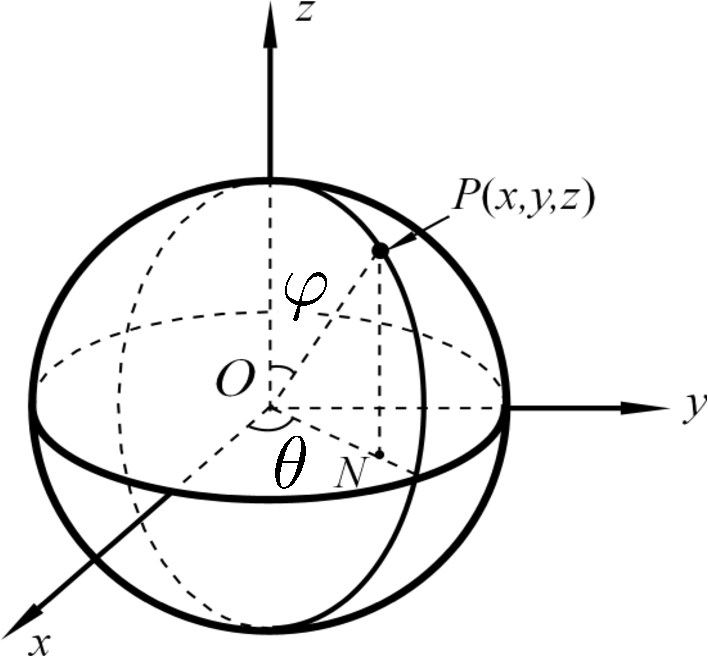
\includegraphics{./images/ch8/sphere.pdf}}
	   	  	\end{center}
	   	\pause
		\column{.5\textwidth}
			$$\alert{\left\{\begin{array}{l}
		  	x=a\sin\varphi\cos\theta,\\
		  	y=a\sin\varphi\sin\theta,\\
		  	z=a\cos\varphi,
			\end{array}\right.}
		  $$
		  
		  $$\alert{\left(\begin{array}{c}
		  	0\leq\theta\leq 2\pi\\
		  	0\leq\varphi\leq\pi
		  \end{array}\right)}$$
	\end{columns}
\end{frame}

\section{旋转曲面}

\begin{frame}{旋转曲面}
	\linespread{1.2}\pause 
% 	曲线绕某直线旋转一周所得的曲面。
	\begin{center}
		\resizebox{!}{2.7cm}{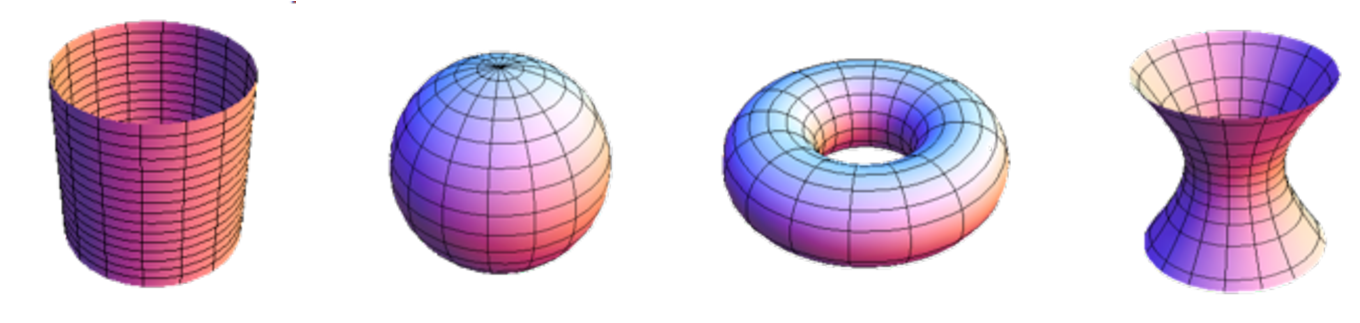
\includegraphics{./images/ch8/twcurve1.pdf}}
	\end{center}\pause 
	\vspace{-1em}
	\begin{exampleblock}{{\bf 例8}\hfill}
		求曲线$C:f(y,z)=0$绕$z$轴旋转一周所得曲面
	\end{exampleblock}\pause 
	\bigskip
	$$\alert{f(\pm\sqrt{x^2+y^2},z)=0}$$
\end{frame}

\begin{frame}{常见的旋转曲面}
	\linespread{1.2}\pause 
	\begin{enumerate}
	  \item {\bf 旋转椭球面:}%$\df{x^2}{a^2}+\df{y^2}{b^2}=1$
	  \begin{center}\pause 
		\resizebox{!}{4.5cm}{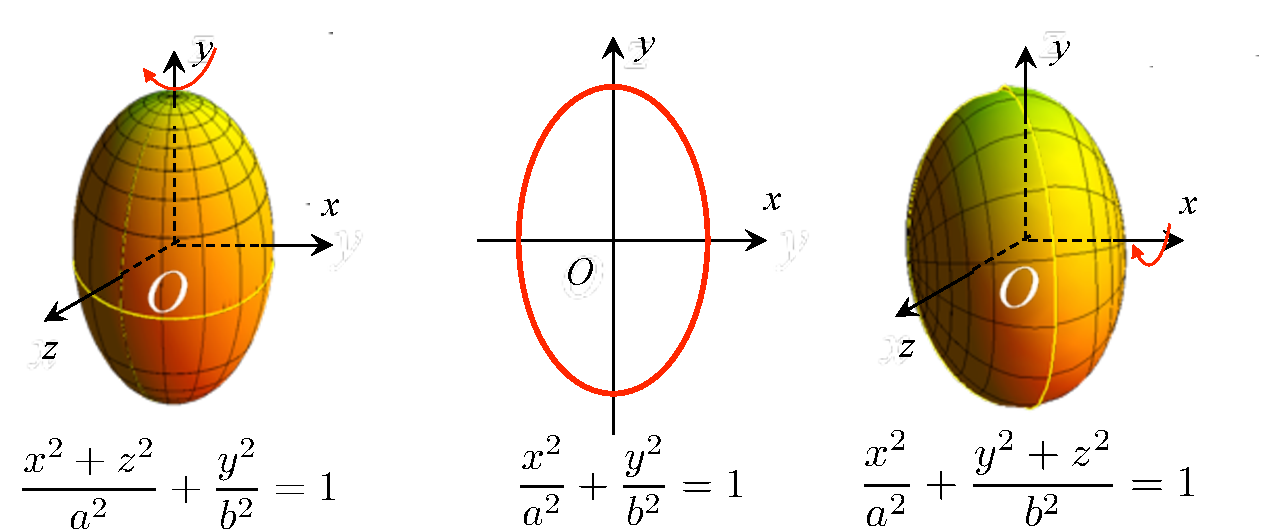
\includegraphics{./images/ch8/rtEllipse.pdf}}
   	  \end{center}
% 	  \item 
	\end{enumerate}
\end{frame}

\begin{frame}
	\linespread{1.2}
	\begin{enumerate}
	  \addtocounter{enumi}{1}
	  \item {\bf 旋转双曲面:}
	  \bigskip\pause 
	  \begin{center}
		\resizebox{!}{4.6cm}{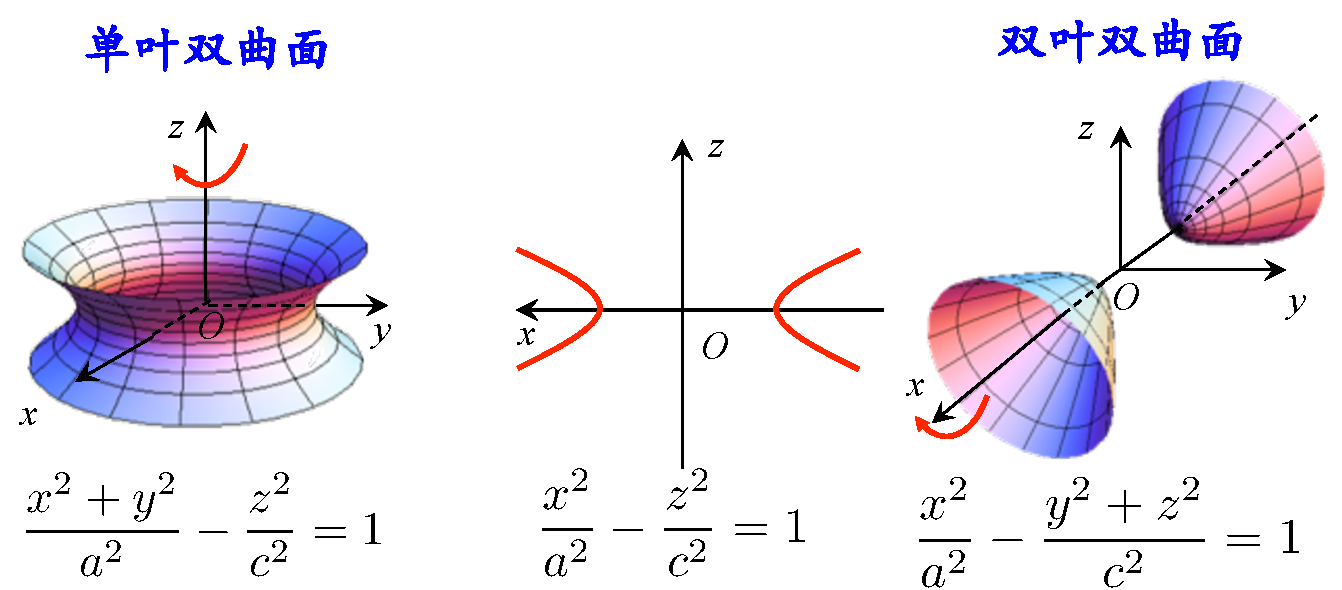
\includegraphics{./images/ch8/rtHypo.pdf}}
   	  \end{center}
% 	  \item 
	\end{enumerate}
\end{frame}

\begin{frame}
	\linespread{1.2}
	\begin{enumerate}
	  \addtocounter{enumi}{2}
	  \item {\bf 旋转抛物面:}
	  \bigskip\pause 
	  \begin{center}
		\resizebox{!}{3.8cm}{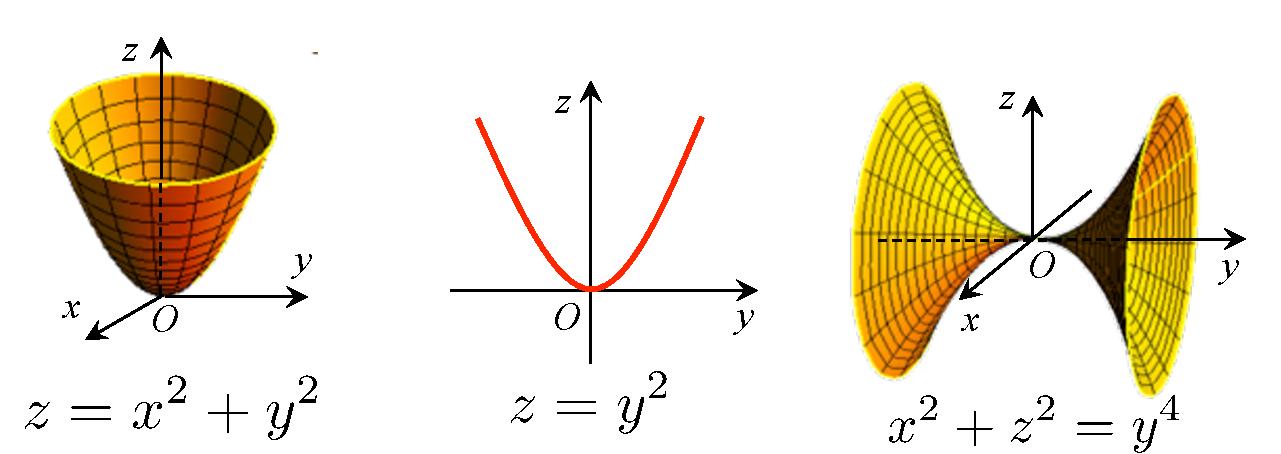
\includegraphics{./images/ch8/rtThc.pdf}}
   	  \end{center}
% 	  \item 
	\end{enumerate}
\end{frame}

\section{柱面}

\begin{frame}{柱面}
	\linespread{1.2}\pause 
	曲线$C:F(x,y)=0$沿$z$轴方向运动的轨迹\pause 
	\begin{center}
		\resizebox{!}{4cm}{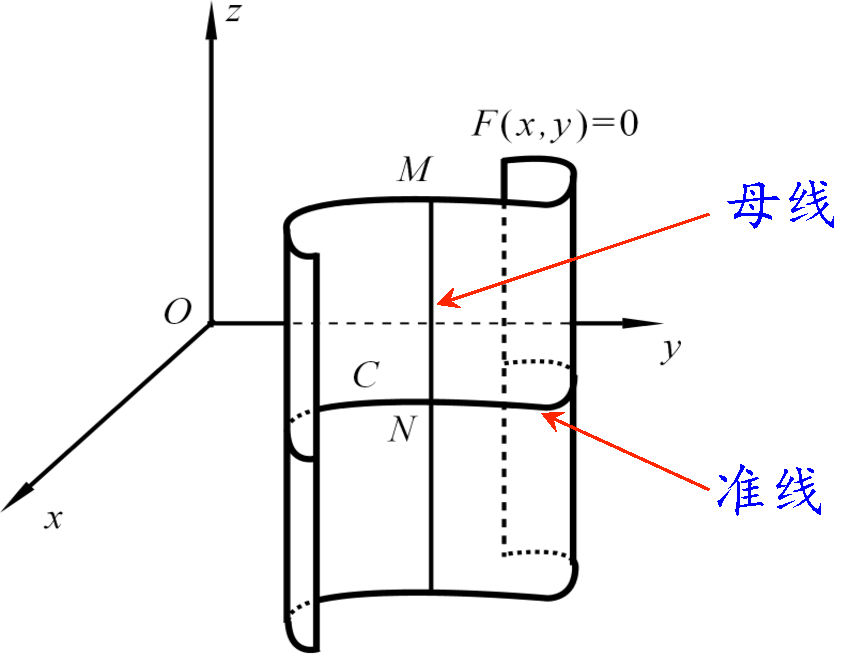
\includegraphics{./images/ch8/cyCurve.pdf}}
 	\end{center}\pause 
	$$\alert{S:\{(x,y,z)\in\mathbb{R}^3|F(x,y)=0\}}$$
\end{frame}

\begin{frame}{常见的柱面}
	\linespread{1.2}\pause 
	\begin{center}
		\resizebox{!}{5cm}{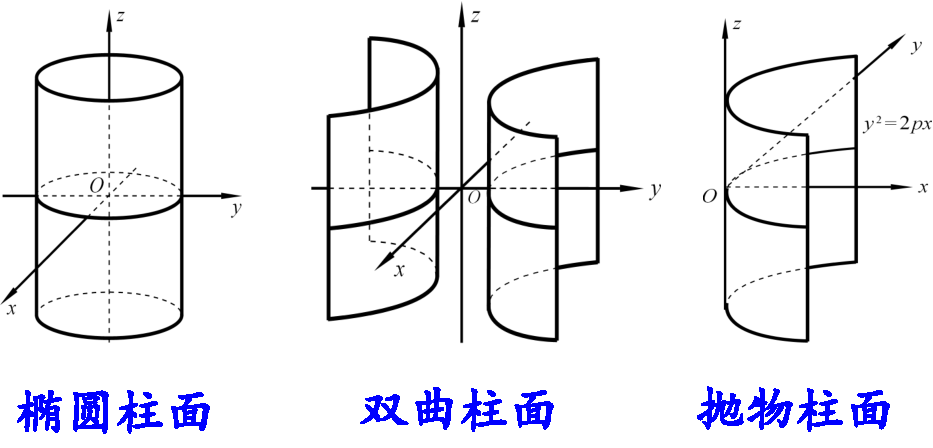
\includegraphics{./images/ch8/cylins.pdf}}
 	\end{center}
\end{frame}

\section{二次曲面}

\begin{frame}{二次曲面}
	\linespread{1.2}\pause 
	\begin{block}{{\bf 定义:}三元二次多项式方程\hfill}
		\vspace{-1em}
		\begin{eqnarray*}
			a_1x^2+a_2y^2+a_3z^2+b_1xy+b_2yx+b_3zx& &\\
			+c_1x+c_2y+c_3z+d & = & 0\\
			(a_1^2+a_2^2+a_3^2\ne 0)& &
		\end{eqnarray*}
	\end{block}\pause 
	{\bf 常见的二次曲面}
	\begin{columns}\pause 
		\column{.5\textwidth}
			\begin{itemize}
			  \item 椭球面\pause 
			  \item 单叶双曲面\pause 
			  \item 双叶双曲面\pause 
			\end{itemize}
		\column{.5\textwidth}
			\begin{itemize}
			  \item 椭圆抛物面\pause 
			  \item 双曲抛物面\pause 
			  \item 椭圆锥面
			\end{itemize}
	\end{columns}
\end{frame}

\begin{frame}{1、椭球面}
	\linespread{1.2}\pause 
	$$\alert{\df{x^2}{a^2}+\df{y^2}{b^2}+\df{z^2}{c^2}=1}$$\pause 
	\begin{center}
		\resizebox{!}{3.5cm}{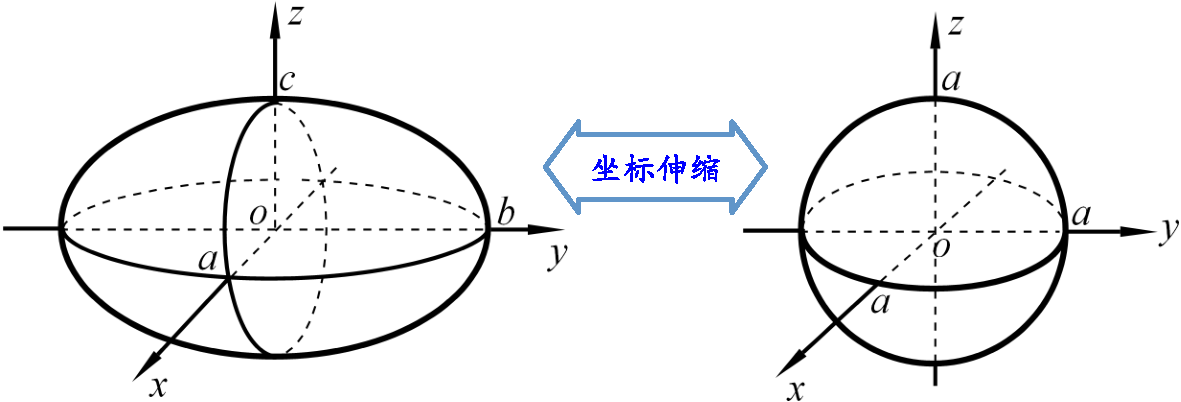
\includegraphics{./images/ch8/quaEllipse.pdf}}
 	\end{center}\pause 
 	$$\alert{x=a\sin\varphi\cos\theta,\;y=b\sin\varphi\sin\theta,\;z=c\cos\varphi}$$
 	$$\alert{(0\leq\theta\leq 2\pi,0\leq\varphi\leq\pi)}$$
\end{frame}

\begin{frame}{2、单叶双曲面}
	\linespread{1.2}\pause 
	$$\alert{\df{x^2}{a^2}+\df{y^2}{b^2}-\df{z^2}{c^2}=1}$$\pause 
	\vspace{-1em}
	\begin{center}
		\resizebox{!}{4cm}{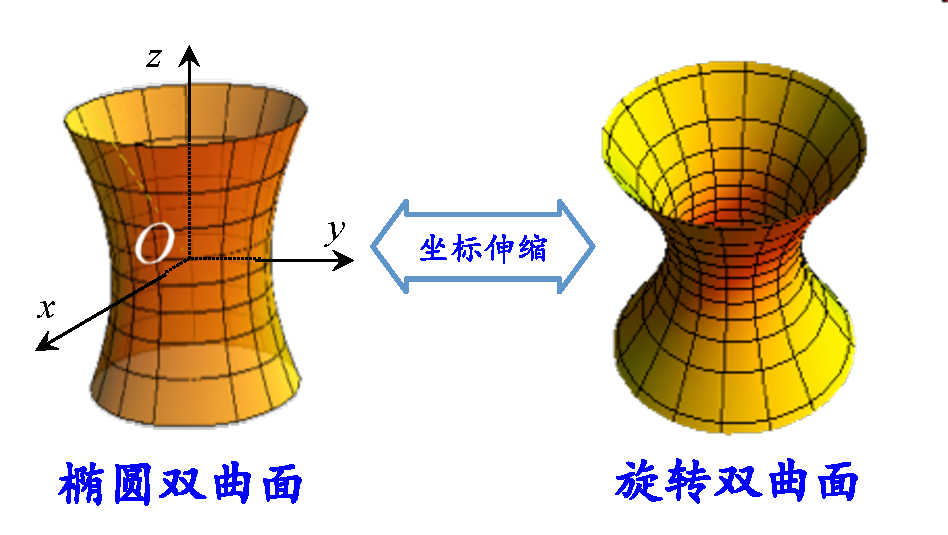
\includegraphics{./images/ch8/quaHypo.pdf}}
 	\end{center}\pause 
 	$$\alert{x=a\sec\varphi\cos\theta,\;y=b\sec\varphi\sin\theta,\;z=c\tan\varphi}$$
 	$$\alert{(0\leq\theta\leq 2\pi,0\leq\varphi\leq\pi)}$$
\end{frame}

\begin{frame}{3、双叶双曲面}
	\linespread{1.2}
	\begin{columns}
		\column{.5\textwidth}
			$$\alert{-\df{x^2}{a^2}-\df{y^2}{b^2}+\df{z^2}{c^2}=1}$$
			\uncover<3->{{\bf 参数方程:}
			$$\alert{\left\{\begin{array}{l}
				x=a\tan\varphi\cos\theta,\\
				y=b\tan\varphi\sin\theta,\\
				z=c\sec\varphi.
			\end{array}\right.}
			$$
			$$\alert{(0\leq\theta\leq 2\pi,0\leq\varphi\leq\pi)}$$}
		\column{.5\textwidth}
		\begin{center}
			\uncover<2->{\resizebox{!}{6.5cm}{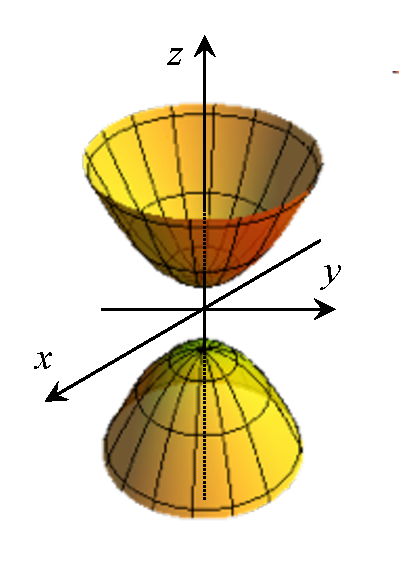
\includegraphics{./images/ch8/quaHypo2.pdf}}}
	 	\end{center}
	\end{columns}
\end{frame}

\begin{frame}{4、椭圆抛物面}
	\linespread{1.2}
	\begin{columns}
		\column{.5\textwidth}
			$$\alert{z=\df{x^2}{a^2}+\df{y^2}{b^2}}$$
			\uncover<3->{{\bf 参数方程:}
			$$\alert{\left\{\begin{array}{l}
				x=au\cos\theta,\\
				y=bu\sin\theta,\\
				z=u^2.
			\end{array}\right.}
			$$
			$$\alert{(0\leq\theta\leq 2\pi,u\geq 0)}$$}
		\column{.5\textwidth}
		\begin{center}
			\uncover<2->{\resizebox{!}{4.5cm}{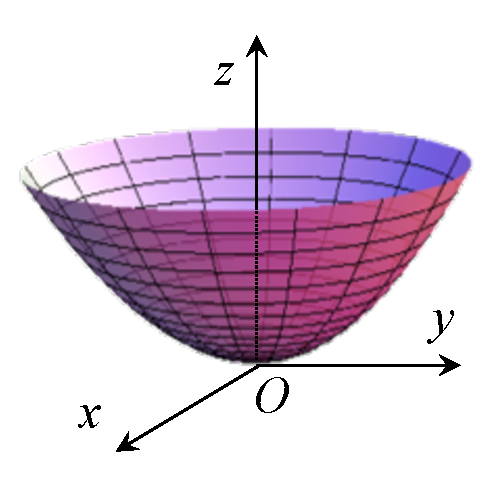
\includegraphics{./images/ch8/quaThr.pdf}}}
	 	\end{center}
	\end{columns}
\end{frame}

\begin{frame}{5、双曲抛物面(马鞍面)}
	\linespread{1.2}\pause 
	$$\alert{z=\df{x^2}{a^2}-\df{y^2}{b^2}}$$\pause 
	\begin{center}
		\resizebox{!}{4cm}{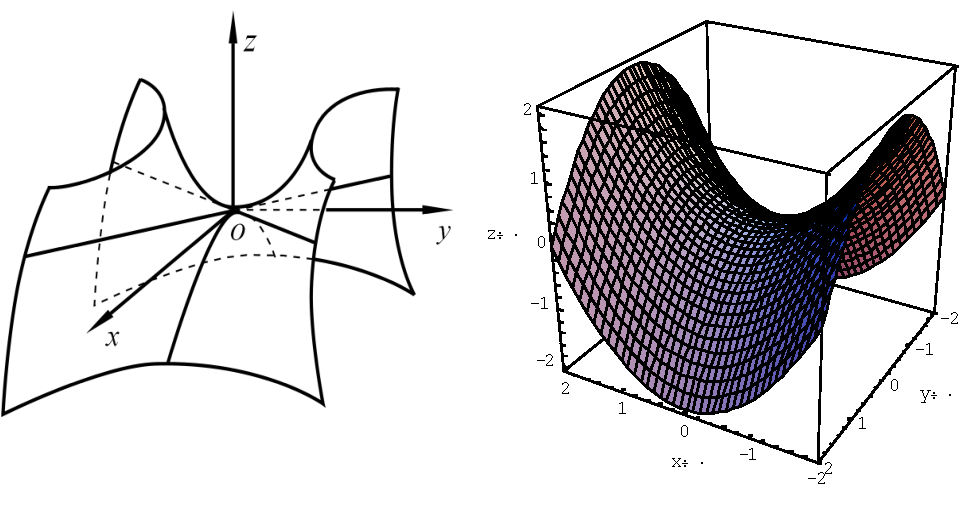
\includegraphics{./images/ch8/quaArch.pdf}}
 	\end{center}\pause 
 	\vspace{-1em}
 	$$\alert{x=au\sec\theta,\;y=bu\tan\theta,\;z=u^2}$$
 	$$\alert{(0\leq\theta\leq 2\pi,u\geq 0)}$$
\end{frame}

\begin{frame}
	\linespread{1.2}
	\begin{exampleblock}{{\bf 例9}\hfill}
		证明:$z=xy$对应的曲面为双曲抛物面
	\end{exampleblock}\pause 
	\begin{center}
		\resizebox{!}{4cm}{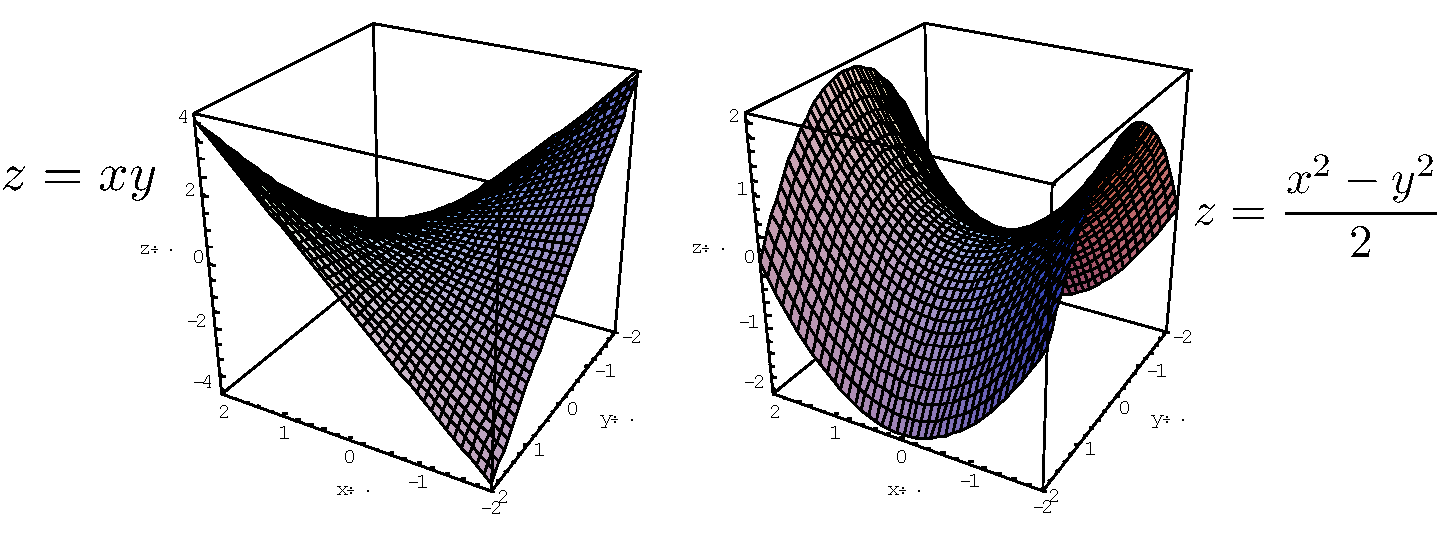
\includegraphics{./images/ch8/diffArch.pdf}}
 	\end{center}\pause 
 	{\bb (二维)坐标旋转公式:}{\b (逆时针旋转$\theta$)}
 	$$\alert{\left\{\begin{array}{l}
 		X=x\cos\theta+y\sin\theta\\
 		Y=-x\sin\theta+y\cos\theta
 	\end{array}\right.}$$
\end{frame}

\begin{frame}{6、椭圆锥面}
	\linespread{1.2}\pause 
	\begin{columns}
		\column{.5\textwidth}
			$$\alert{\df{x^2}{a^2}+\df{y^2}{b^2}-\df{z^2}{c^2}=0}$$\pause 
			{\bf 参数方程:}
			$$\alert{\left\{\begin{array}{l}
				x=au\cos\theta,\\
				y=bu\sin\theta,\\
				z=u.
			\end{array}\right.}
			$$
			$$\alert{(0\leq\theta\leq 2\pi,u\in\mathbb{R})}$$
		\column{.5\textwidth}\pause 
		\begin{center}
			\resizebox{!}{6cm}{\includegraphics{./images/ch8/quaCone.pdf}}
	 	\end{center}
	\end{columns}
\end{frame}

\begin{frame}[<+->]{小结}
	\linespread{1.5}
	\begin{enumerate}
	  \item {\bf 曲面方程及其参数化}
	  \begin{itemize}
	    \item 曲面参数方程需要两个参数
	  \end{itemize}
	  \item {\bf 旋转曲面与柱面}
	  \item {\bf 二次曲面}
	  \begin{itemize}
	    \item 标准方程
	    \item 参数方程
	  \end{itemize}
	\end{enumerate}
\end{frame}

\begin{frame}{直纹面}
	\linespread{1.2}
	\ba{空间直线按照一定的规律运动会产生什么样的曲面?}\pause 
	\begin{center}
		\resizebox{!}{5cm}{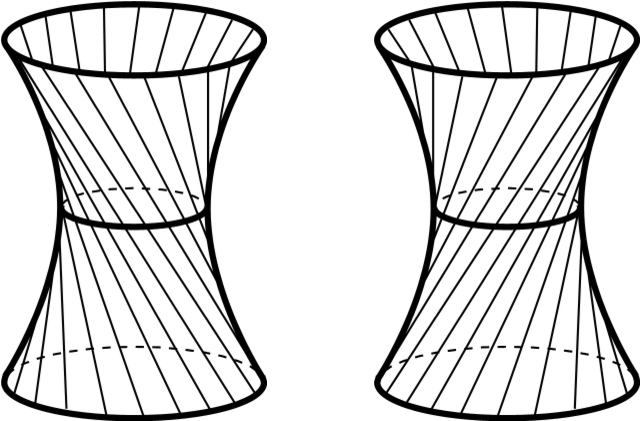
\includegraphics{./images/ch8/rtLHypo.pdf}}
		
		{\b 单叶双曲面}
 	\end{center}
\end{frame}

\begin{frame}[<+->]
	\linespread{1.2}
	\begin{exampleblock}{{\bf 例10:}判断以下曲面的类型及其特征\hfill}
		\begin{columns}[t]
			\column{.55\textwidth}
				\begin{enumerate}
				  \item $x^2+y^2+z^2+2x-2y=0$
				  \item $x^2-y^2+z^2+2x-2y=0$
				  \item $x^2+y^2+z^2+2x-2y=2$
				  \item $x^2-y^2+z^2+2x-2y=2$
				  \item $x^2-y^2+z^2+2x-2y=-2$
				  \item $x^2+y^2+z^2+2x+2y=2$
				\end{enumerate}
			\column{.45\textwidth}
				\begin{enumerate}
				  \addtocounter{enumi}{6}
				  \item $x^2+y^2-z^2+2xy=0$
				  \item $x^2+y^2-z=0$
				  \item $x^2-y^2-z=0$
				  \item $x^2-z=0$
				  \item $x^2-y+z=0$
				\end{enumerate}
		\end{columns}
	\end{exampleblock}
\end{frame}

% \begin{frame}{title}
% 	\linespread{1.2}
% 	\begin{block}{{\bf title}\hfill}
% 		123
% 	\end{block}
% \end{frame}